\documentclass[english, apj]{emulateapj}
\usepackage[T1]{fontenc}
\usepackage[latin9]{inputenc}
\usepackage{array}
\usepackage{rotating}
\usepackage{units}
\usepackage{textcomp}
\usepackage{amsmath}
\usepackage{amsbsy}
\usepackage{amstext}
\usepackage{graphicx}
\usepackage{url}
\usepackage{babel}
%\usepackage{siunitx}
%\sisetup{output-exponent-marker=\ensuremath{\mathrm{e}}}
\usepackage[backref,breaklinks,colorlinks,citecolor=blue]{hyperref}
\usepackage[all]{hypcap}

\makeatletter

\newcommand{\msun}{\mbox{$\,{\rm M}_\odot$}}

\sloppy

\providecommand{\tabularnewline}{\\}

\begin{document}

\title{Cannibalism among the supermassive black holes}


\author{Charles Zivancev\altaffilmark{1}, Andreas H.W. K\"upper\altaffilmark{1,2}, Jeremiah P. Ostriker\altaffilmark{1,3}}
\altaffiltext{1}{Department of Astronomy, Columbia University, 550 West 120th Street, New York, NY 10027, USA}
\altaffiltext{2}{Hubble Fellow}
\altaffiltext{3}{Princeton University, New Jersey, USA}
\email{Correspondence to: csz2104@columbia.edu}




\begin{abstract}

\end{abstract}


\keywords{Galaxy: kinematics and dynamics}




\section{Introduction}\label{sec:introduction}
A majority of all galaxies with masses $>10^8\msun$ at $z=0$ are believed to host super-massive black holes (SMBHs) in their cores. In a $\Lambda$CDM universe, galaxies at the high end of the galaxy-mass function are merger products of tens to hundreds of such massive galaxies. Even if only a small fraction of merging galaxies hosted an SMBH in their core at the time of merging, it is reasonable to assume that, during a Hubble time of continuous growth, these galaxies they will have substantial phases in which they contain two or more SMBHs at the same time. 

Here we look at the merger history of four exemplary galaxies across the galaxy mass spectrum extracted from a cosmological simulation of hierarchical structure formation. We investigate how, after merging with incoming galaxies, SMBHs diffuse into the cores of the hosts and interact with the resident black hole. We show that gravitational interactions of multiple SMBHs is most probable in high-mass galaxies with $10^{12}<M/\msun < 10^{13}$. Galaxies with lower masses  have too few mergers with SMBH hosting galaxies. Galaxies with higher masses tend to be too extended, making dynamical friction processes inefficient and hence failing to drive SMBHs into the host galaxy core.

This paper is organized as follows: in Section \ref{sec:methods} we are going to describe the cosmological simulation from which we use the merger history to setup our idealized numerical simulations. We present the few-body integration code, \textsc{AR-Chain} that we used for our simulations of SMBH dynamics, and the modifications we made to this code in order to deal with a host galaxy's gravitational potential. In Section \ref{sec:results}, we show the results of our four exemplary simulations of galaxies growing with time and acquiring new SMBHs. We analyze how the SMBHs are driven into the core of their new host galaxies and how interaction with the host black hole leads to near-ejections or mergers. The final Section \ref{sec:conclusions} contains a discussion of the result and our conclusions.


\section{Methods}\label{sec:methods}
\begin{figure*}[htbp]
\begin{center}
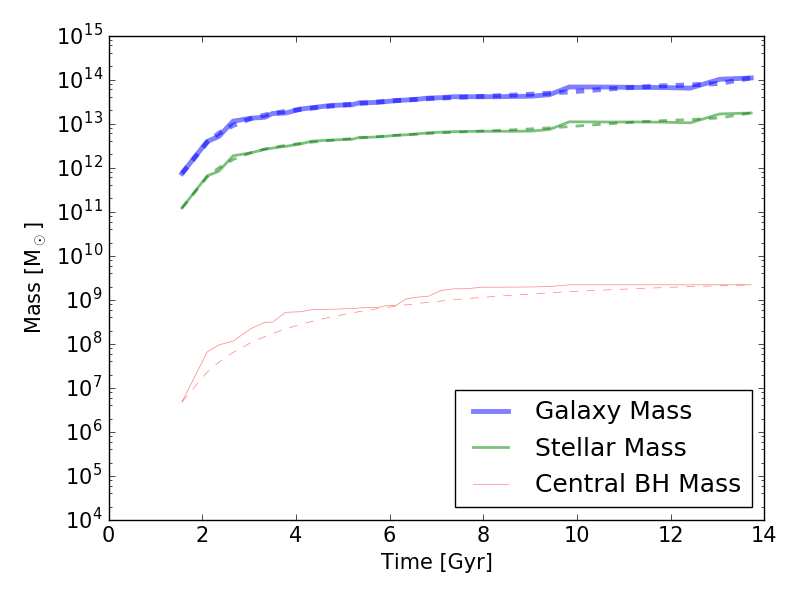
\includegraphics[width=0.45\textwidth]{plots/Masses_plot_galaxy_1.png}
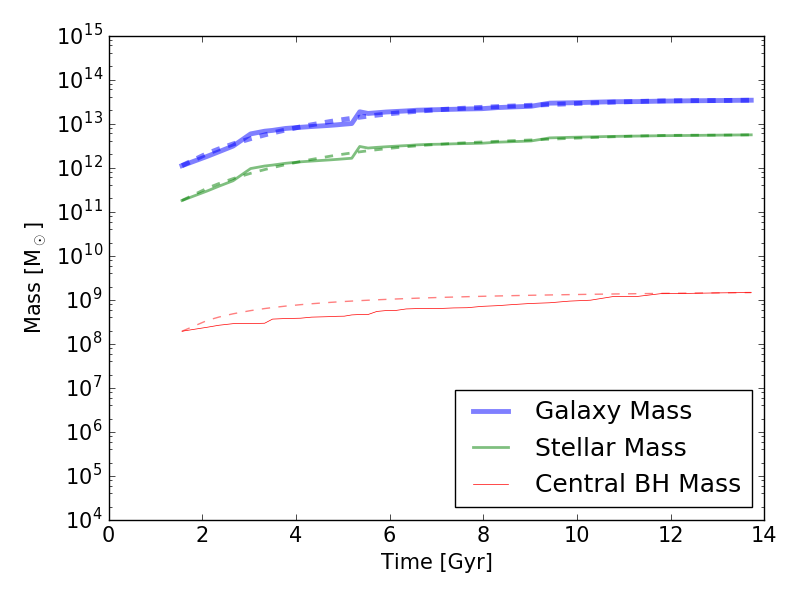
\includegraphics[width=0.45\textwidth]{plots/Masses_plot_galaxy_65.png}\\
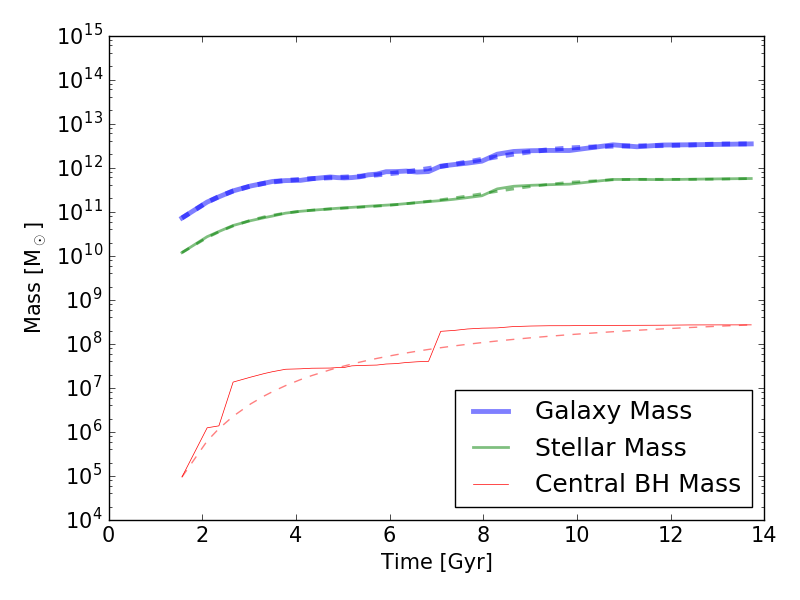
\includegraphics[width=0.45\textwidth]{plots/Masses_plot_galaxy_187.png}
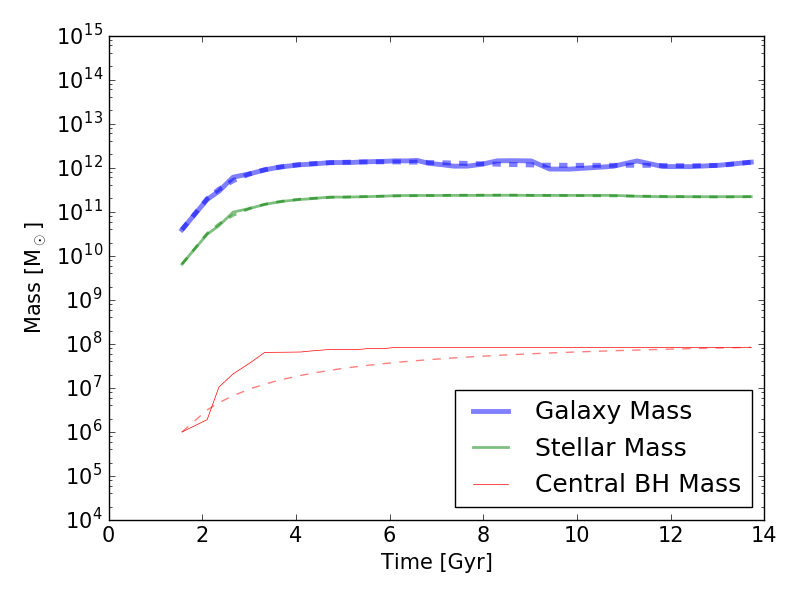
\includegraphics[width=0.45\textwidth]{plots/Masses_plot_galaxy_217.png}\\
\caption{default}
\label{default}
\end{center}
\end{figure*}


\subsection{Merger tree}
Our merger tree data came from the SMBH evolution simulations of \citet{2015ApJ...799..178K}, which used the large-scale hydrodynamical galaxy simulations outlined in \citet{2011ApJ...741...99C, 2011ApJ...742L..33C, 2012ApJ...753...17C, 2012ApJ...748..121C, 2013ApJ...770..139C}.  The following cosmological parameters were used in their simulation:   $\Omega_M = 0.28$, $\Omega_b = 0.046$, $\Omega_\Lambda = 0.72$, $\sigma_8 = 0.82$, $H_0 = 100h^{-1}Mpc^{-1} = 70 km s^{-1} Mpc^{-1}$, and $n = 0.96$.  The SMBHs were evolved from $4\geq z \geq 0$.

The merger tree data was in two primary files.  One file was centered around SMBHs at each redshift slice, giving information for the black hole's seed mass, accreted and seed mass, its host galaxy, the stellar mass in its host galaxy, and time after z=4 at which the BH entered the host galaxy (if it is not the central BH).  The other file was centered on galaxies at each redshift slice, prociding information on the galaxyies' stellar mass, dark matter mass, its central BH, and any orbiting black holes within the galaxy.

Starting with this data, we plotted the galaxy masses as a function of time.  Since the raw data was given in terms of redshift, we converted redshift to time with the help of a 'cosmology calculator', courtesy of Ned Wright and James Schombert (\url{http://www.astro.ucla.edu/~wright/CosmoCalc.html}).  We chose four galaxies to run our simulations.  The galaxies were chosen using the following basic criteria:
\begin{itemize}
\item The galaxies had to exist through the entire simulation, from $z=4$ to $z=0$.
\item They had to have a central SMBH.
\item They had to have at least XXX orbiting black holes.
\item We ordered the galaxies by decreasing mass at $z=0$, and starting with the largest tier of mass (~$10^{14} M_{\odot}$), we spaced their masses by approximately 1-2 orders of magnitude.
\end{itemize}

After finding our subject galaxies, we curve-fit their total masses as a function of time using a simple $7^{th}$-order polynomial fit, so as to be able to use their masses in the AR-Chain code.  Additionally, we curve-fit each galaxy's accreted+seed central black hole mass to exponential functions of time.

\subsection{AR-Chain code}
Summary of the code and the modifications we made.

For the numerical simulations presented here, we used a modified version of the algorithmic chain integrator \textsc{AR-Chain} developed by \citet{2006MNRAS.372..219M}. It uses algorithmic chain regularization for high-precision integration of few-body dynamics, and is capable of handling velocity-dependent forces efficiently. It includes relativistic post-Newtonian terms up to order PN2.5 \citep{2008AJ....135.2398M}.


\subsubsection{Galaxy background potential}
The simulations from which we obtained the merger tree data considered only dark matter distributions and were run using the Navarro-Frenk-White (NFW) profile described in \citet{1997ApJ...490..493N}.  Since our study is more interested SMBH mergers at the center of galaxies, dynamical friction, and hence baryonic matter, was of considerable importance.  Therefore, NFW background potential was less suitable for our application.

In considering a suitable potential-density pair, characteristics that were important were:
\begin{itemize}
\item It must take into account baryonic matter
\item It must have a finite density in the center out to a scale radius
\item Declining density that drops more sharply out to a second scale radius
\item An even sharper decline in density beyond the second scale radius
\item It must be easily parametrized and written in analytic, closed form
\end{itemize}

For our simulations, the Jerry profile (\citet{2015ApJ...806L..28S}), which is a three-parameter potential-density pair, was used.  In order to fully parametrize the Jerry profile so as to use it in our simulations, we needed to match the stellar and halo mass data from the Kulier et al simulations, to the velocity dispersion at the galaxy's effective radius.  In Kulier's simulations, a galaxy's effective radius $R_{e}$ and velocity dispersion $\sigma(R_e)$ at the effective radius are:
\begin{equation} \label{re}
R_{e} = 2.5 kpc\left(\frac{M_*}{10^{11}M_{\odot}}\right)^{0.73}(1+z)^{-0.98}
\end{equation}
\begin{equation} \label{sig}
\sigma(R_{e}) = 190km/s\left(\frac{M_{*}}{10^{11}M_{\odot}}\right)^{0.2}(1+z)^{0.47}
\end{equation}

Given the galaxy's stellar mass $M_{*}$ at redshift z from Kulier's simulations, we can calculate the effective radius and velocity dispersion.  We can then equate these values to the analytic expressions for $\sigma(R_{e})$ in the Jerry profile.  Using a core radius $r_c$ = 100, we can solve for the halo radius $r_h$ using a simple recursive Newton method.  Whether $\sigma_{near}$ or $\sigma_{far}$ is used is determined by whether $R_e$ is less than or greater than $\sqrt{r_c r_h}$.

\subsubsection{Phase-space diffusion}
Weak encounters with background stars will let the SMBHs diffuse through phase space while they are orbiting within the gravitational potential of the galaxy.

\subsubsection{Gravitational wave recoils}
The code \textsc{AR-Chain} includes PN terms up to order 2.5. The SMBHs can therefore merge via gravitational wave emission. We include gravitational wave recoils following the prescription outlined in \citet{2015ApJ...799..178K}, which is based on the fitting formula by \citet{2012PhRvD..85h4015L}. To save computational time, we assume that a merger will be inevitable when the separation between two SBHs gets smaller than 10\,000 Schwarzschild radii. At the moment of the merger, we assume that the spin vectors of the two SBHs are randomly aligned. This results in kick velocities of up to several thousand km\,s$^{-1}$, with a median kick of $\approx 290$\,km\,s$^{-1}$. Since our simulations focus on NSC with relatively low escape velocities, this implies that a majority of the merging SBHs escape from the NSCs. 

Black holes can also eject each other via strong three-body interactions. We remove SBHs from the simulations once they move beyond 1\,kpc from the NSC, assuming that it will take them more than a Hubble time to find their way back into the center of the host galaxy.


\subsection{Simulation setup}
Injection, merging, escape, effective radius, set of galaxies

Using the merger tree data, orbiting black holes were injected into its host galaxy at redshift z, at a distance from the galactic center of $R_{e}$ (Eqn. \ref{re}).  Their initial velocity was arbitrarily chosen to be circular, $v_c = \sqrt{M(R_e)/R_e}$, with $v_x$, $v_y$, and $v_z$ randomly chosen.

Note: we only inject the BHs into the simulation that have a $t_{fric}$ smaller than 100 times the Hubble time.


\subsection{Description of Simulations}
\begin{table*}
\centering
\caption{Galaxy characteristics}
\begin{tabular}{c| c c| c c| c c}
 & \multicolumn{2}{c}{$M_{gal}$ [$M_{\odot}$]} & 
\multicolumn{2}{c}{$M_{*}$ [$M_{\odot}$]} & 
\multicolumn{2}{c}{$M_{BH}$ [$M_{\odot}$]} \\
\hline
Galaxy & Init & Final & Init & Final & Init & Final \\
 \hline
A & $7.42\times10^{11}$ & $1.09\times10^{14}$  & $1.22\times10^{11}$ & $1.75\times10^{13}$ & $4.80\times10^{6}$ & $2.19\times10^{9}$\\
B & $1.11\times10^{12}$ & $3.41\times10^{13}$ & $1.80\mathrm{3}{11}$ & $5.58\times10^{12}$ & $1.94\times10^{8}$ & $1.46\times10^{9}$\\
C & $7.23\times10^{10}$ & $3.48\times10^{12}$ & $1.18\times10^{10}$ & $5.68\times10^{11}$ & $9.47\times10^{4}$ & $2.70\times10^{8}$\\
D & $3.92\times10^{10}$ & $1.34\times10^{12}$ & $6.47\times10^{9}$ & $2.20\times10^{11}$ & $9.95\times10^{5}$ & $8.32\times10^{7}$\\
\end{tabular}
\end{table*}





\section{Results}\label{sec:results}
\begin{table*}
\centering
\caption{SMBH statistics}
\begin{tabular}{c| c |c |c}
Galaxy & Infalling SMBHs & SMBHs with $t_{fric}<100\,t_H$ & Mergers \\
\hline
A & 206 & 19 & 4 \\
B & 29 & 12 & 4 \\
C & 3 & 3 & 2 \\
D & 4 & 4 & 2 \\
\end{tabular}
\end{table*}

\begin{figure*}[htbp]
\begin{center}
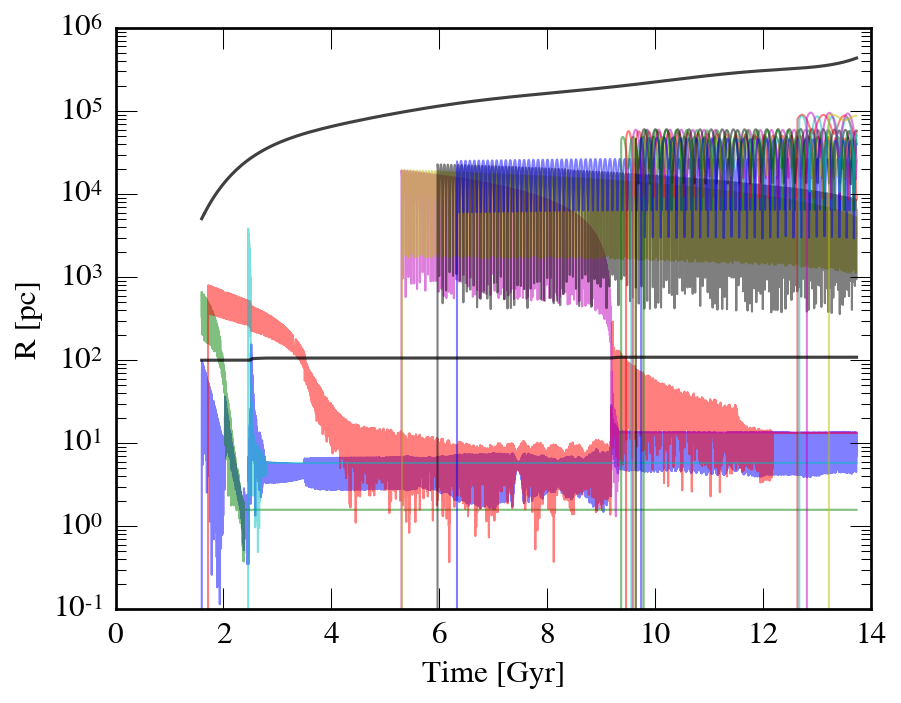
\includegraphics[width=0.45\textwidth]{plots/radius_A.png}
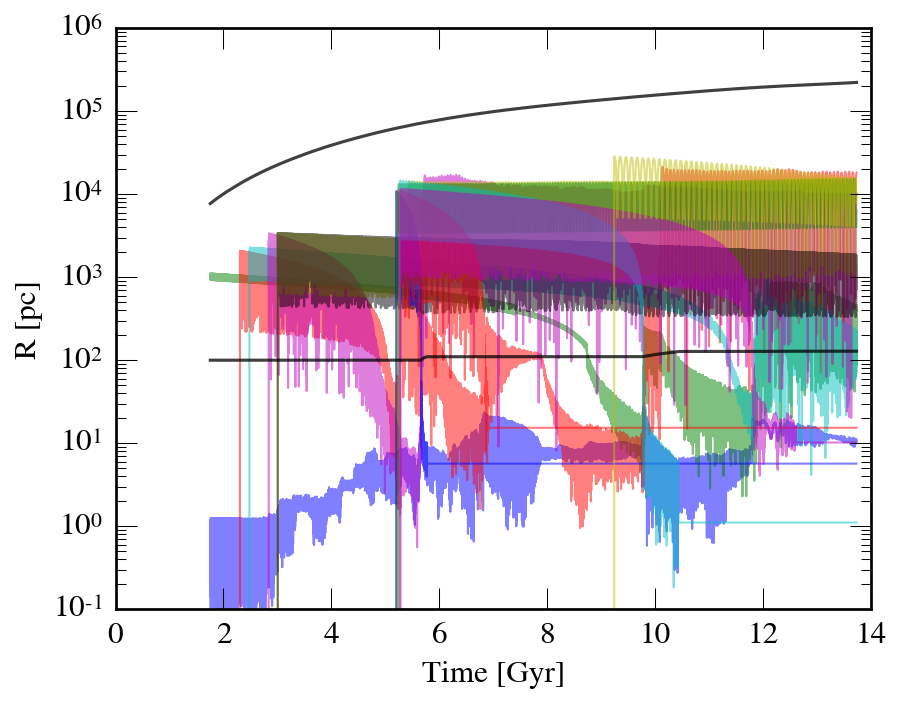
\includegraphics[width=0.45\textwidth]{plots/radius_B.png}\\
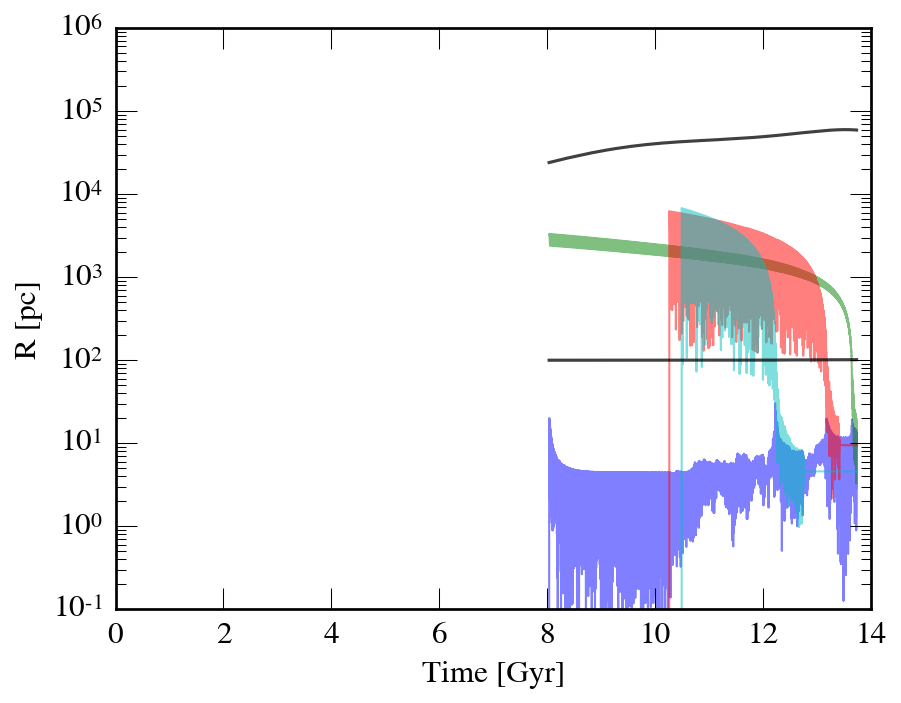
\includegraphics[width=0.45\textwidth]{plots/radius_C.png}
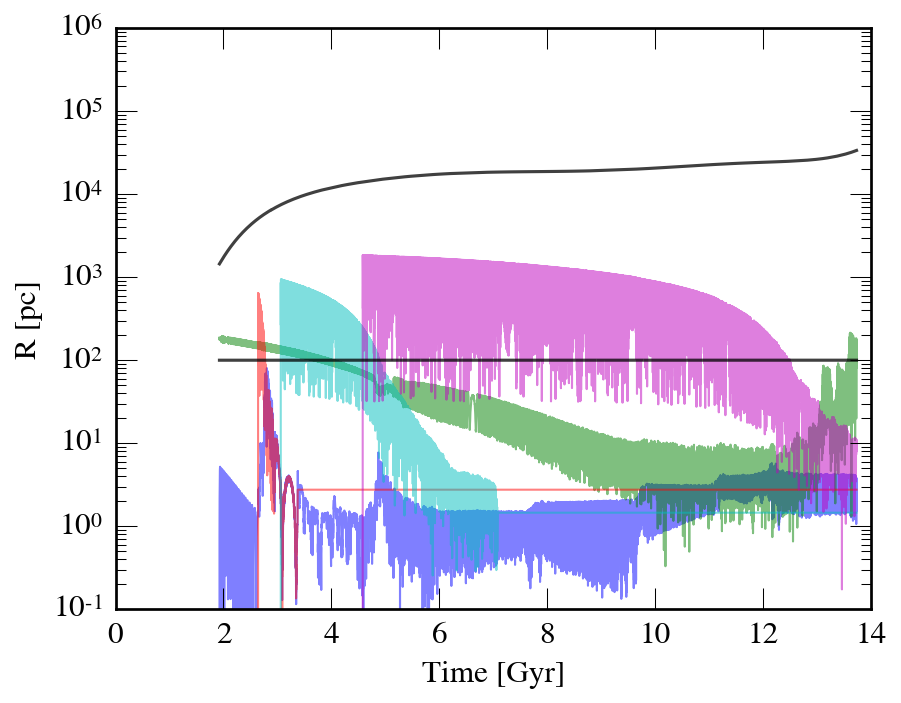
\includegraphics[width=0.45\textwidth]{plots/radius_D.png}\\
\caption{default}
\label{default}
\end{center}
\end{figure*}

\begin{figure*}[htbp]
\begin{center}
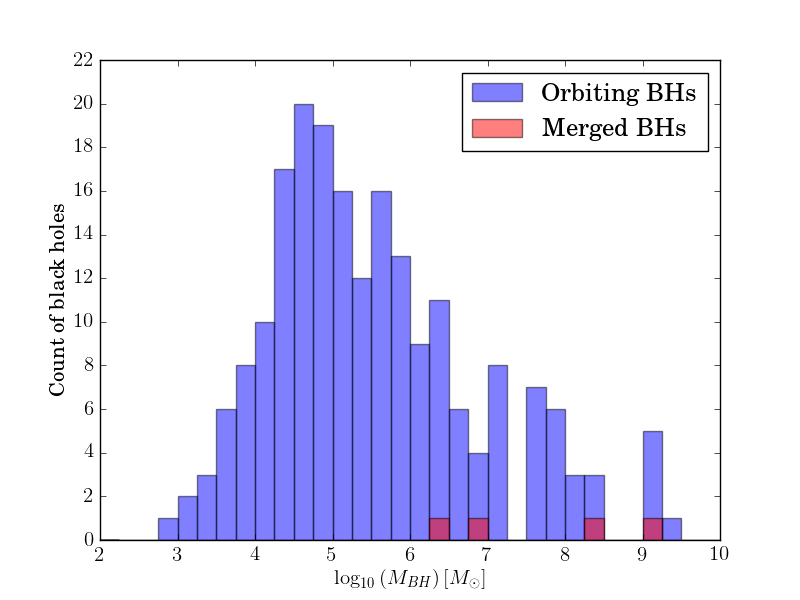
\includegraphics[width=0.45\textwidth]{plots/orbiting_bh_mass_histogram_gal_1.png}
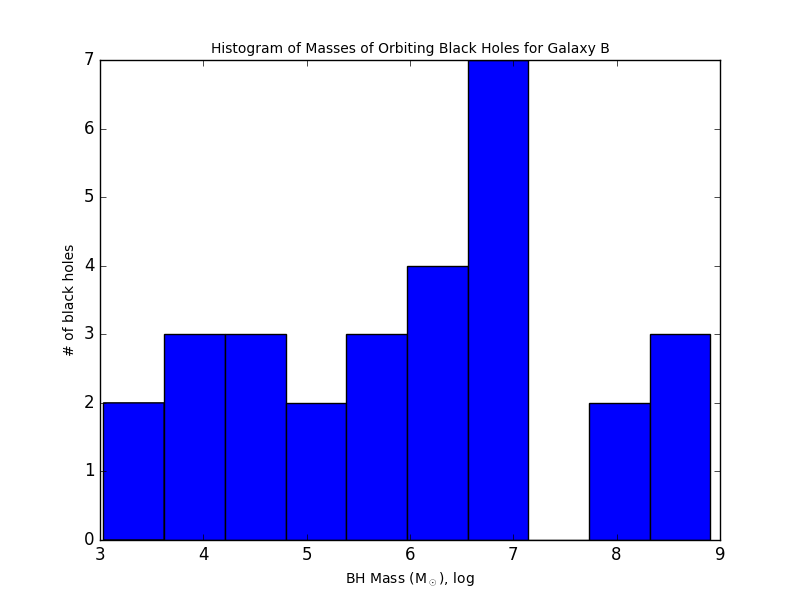
\includegraphics[width=0.45\textwidth]{plots/orbiting_bh_mass_histogram_gal_65.png}\\
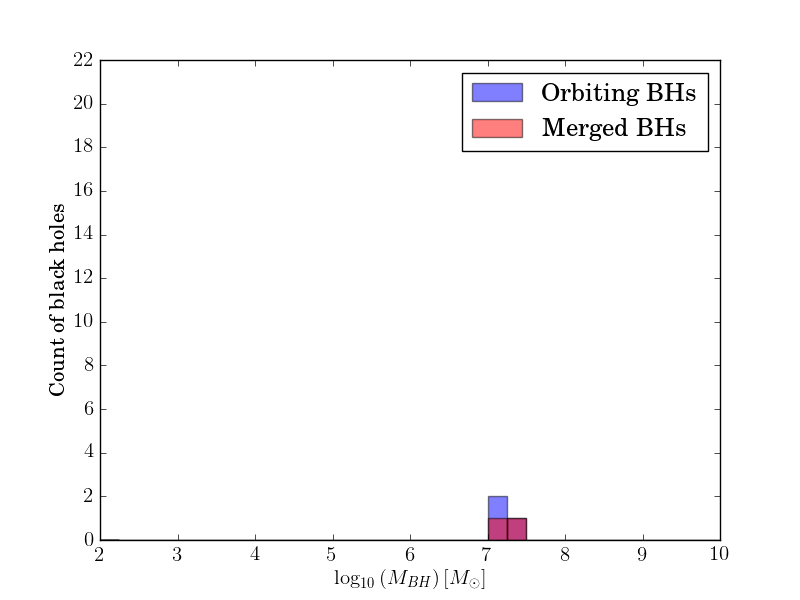
\includegraphics[width=0.45\textwidth]{plots/orbiting_bh_mass_histogram_gal_187.png}
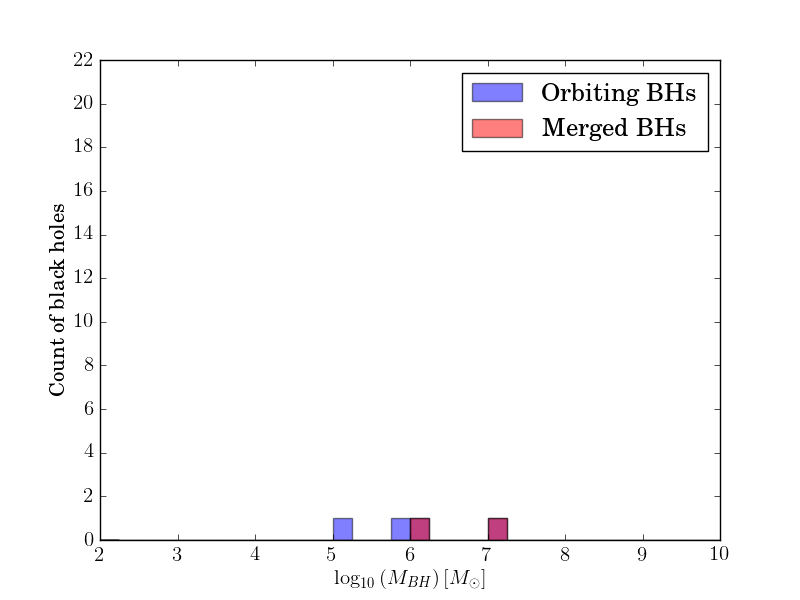
\includegraphics[width=0.45\textwidth]{plots/orbiting_bh_mass_histogram_gal_217.png}\\
\caption{default}
\label{default}
\end{center}
\end{figure*}

\subsection{Mergers}
\begin{figure}[htbp]
\begin{center}
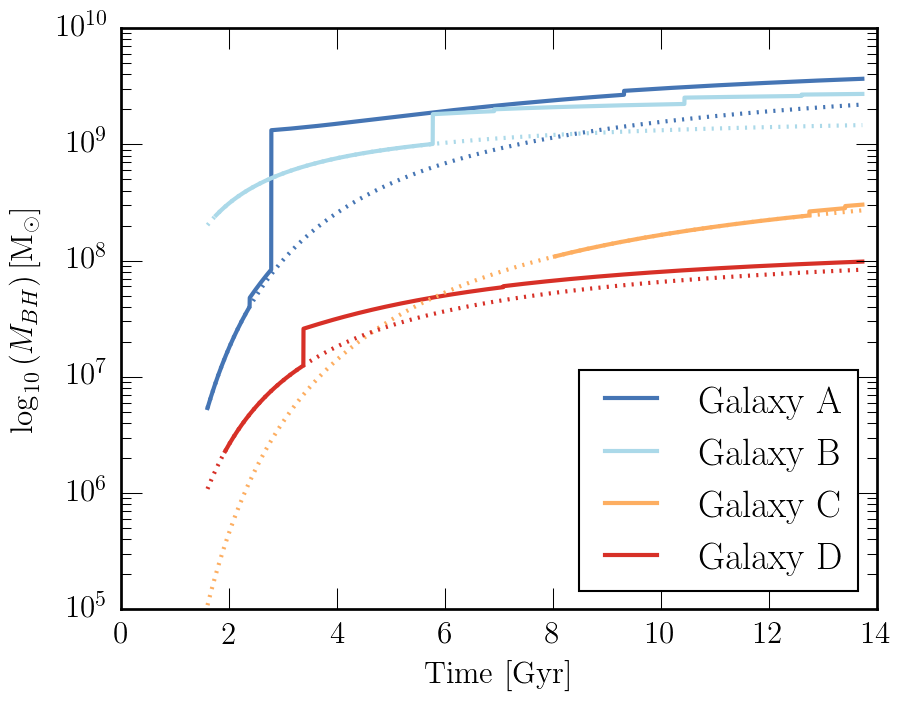
\includegraphics[width=0.45\textwidth]{plots/masses_ABCD.png}
\caption{default}
\label{default}
\end{center}
\end{figure}




\noindent A: two mergers early on, and then two more at around 10-12 Gyr\\
B: 4 mergers across the final 8 Gyr\\
C: two mergers in the final Gyrs\\
D: ?\\


\subsection{Ejections}
No complete ejections, but kicks to higher energy orbits.
\noindent A: one in a three-body encoutner\\
B: 7-ish kicks, some in nearly 4-body encounters\\
C: none\\
D: ?\\

\subsection{Stalling SMBH binaries}
A: two periods of BH binary in center for > Gyr, up to 6 Gyr\\
B: two short periods of BHBs\\
C: 2 classic BHB periods of about 1 Gyr each\\
D: ?

\subsection{Stalling SMBHs in the halo}
\begin{figure*}[htbp]
\begin{center}
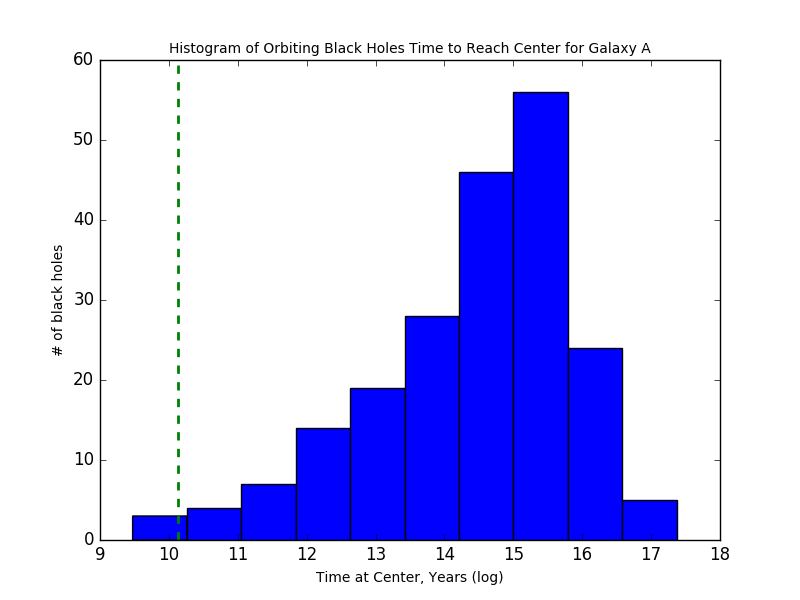
\includegraphics[width=0.45\textwidth]{plots/t_at_center_histogram_gal_1.png}
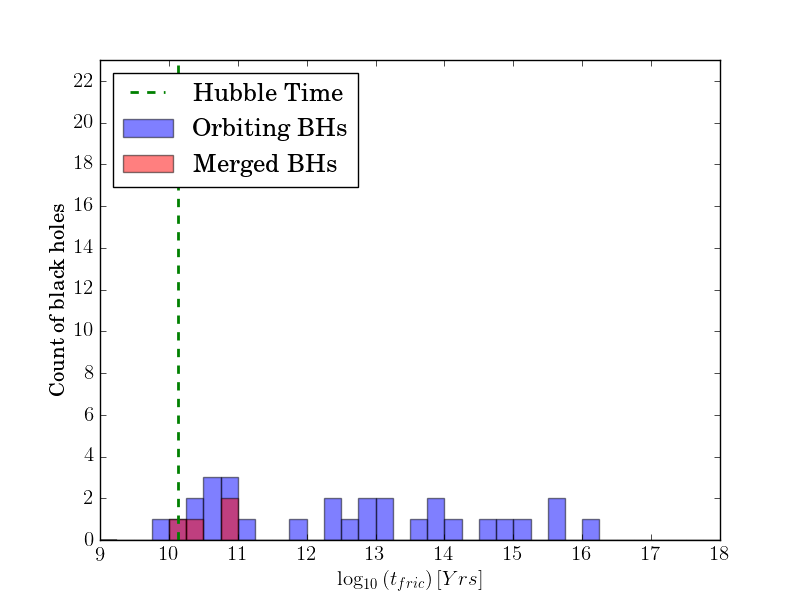
\includegraphics[width=0.45\textwidth]{plots/t_at_center_histogram_gal_65.png}\\
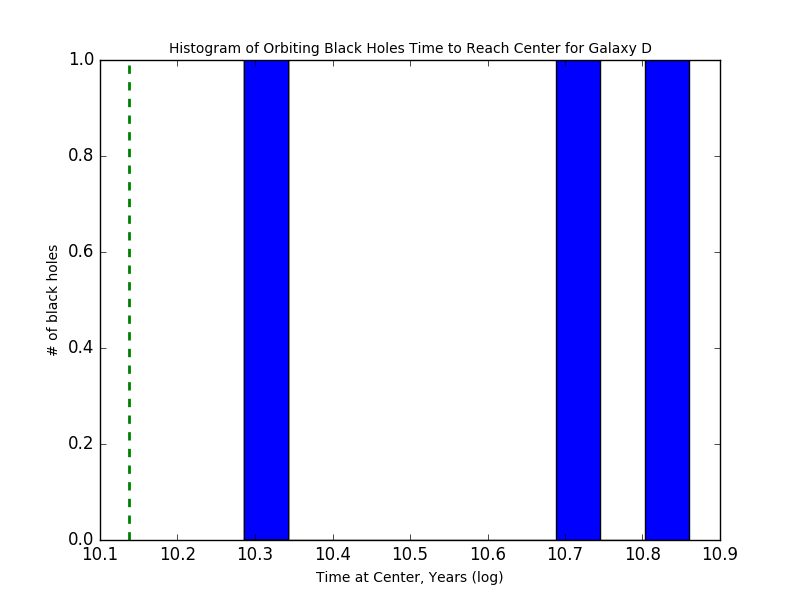
\includegraphics[width=0.45\textwidth]{plots/t_at_center_histogram_gal_187.png}
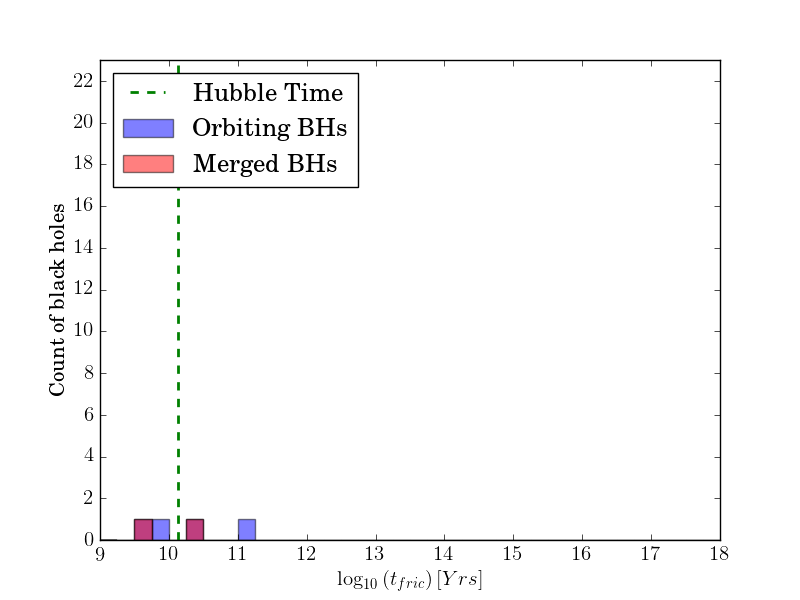
\includegraphics[width=0.45\textwidth]{plots/t_at_center_histogram_gal_217.png}\\
\caption{default}
\label{default}
\end{center}
\end{figure*}

A: 95\% never make it into the central kpc\\
B: still about 90\% are in the halo\\
C: \\
D: ?



\section{Conclusions}\label{sec:conclusions}
What do we want to say?



\section*{Acknowledgements}

The authors would like to thank Andrea Kulier for providing merger tree data. AHWK acknowledges support by NASA through Hubble Fellowship grant HST-HF-51323.01-A awarded by the Space Telescope Science Institute, which is operated by the Association of Universities for Research in Astronomy, Inc., for NASA, under contract NAS 5-26555. 

\bibliographystyle{apj}
\bibliography{biblio}

%\begin{thebibliography}{}

%\bibitem[\protect\citeauthoryear{Aarseth}{2003}]{Aarseth03}
%Aarseth, S.~J., 2003, Gravitational N-Body Simulations (Cambridge University Press)


%\bibitem[\protect\citeauthoryear{K{\"u}pper et al.}{2011}]{Kupper11} 
%K{\"u}pper, A.~H.~W., Maschberger, T., Kroupa, P., Baumgardt, H., 2011, MNRAS, 417, 2300 

%\end{thebibliography}
\end{document}

